
\section{Ground Motion Simulation Results}

Before we address the evaluation of the models, we present results from the simulations and offer a general perspective on the ground motion characteristics obtained for the events considered. Fig.~\ref{fig:all.pgvs} shows the peak horizontal magnitude of velocity on the free surface for all events, and for the particular case of simulations done using the model CVM-S4.26. This figure illustrates how the basins in the region respond to earthquakes originated at various locations within the simulation domain. Although interpretations in this regard are biased by the choice of the color scale, it is fair to say that earthquakes of magnitude less than 3.9 remain local, showing only a marginal ground response in areas outside their immediate epicentral surrounding (e.g.~events L, M, U). Events of magnitude greater than 4.3, on the other hand, show stronger response all throughout the domain, and exhibit more clearly the effects of the basins (e.g.~events D, P, Y). Events with magnitudes between 3.9 and 4.3 are in a transition zone. In such cases the shallower events register stronger ground motions (e.g.~events Q and Z). 

All events considered, the largest ground motions are obtained for the 2014 \eqmag{w} 5.10 La Habra and 2008 \eqmag{w} 5.39 Chino Hills earthquakes (events W and X, respectively), and the areas with most significant shaking are the greater Los Angeles basin, the San Bernardino basin and the region between Simi valley and the Ventura basin. While Fig.~\ref{fig:all.pgvs} only includes results obtained using CVM-S4.26, these observations are consistent across velocity models. We, however, now focus our attention to the discrepancies observed when using different velocity models. 

\begin{figure*}
    \centering
    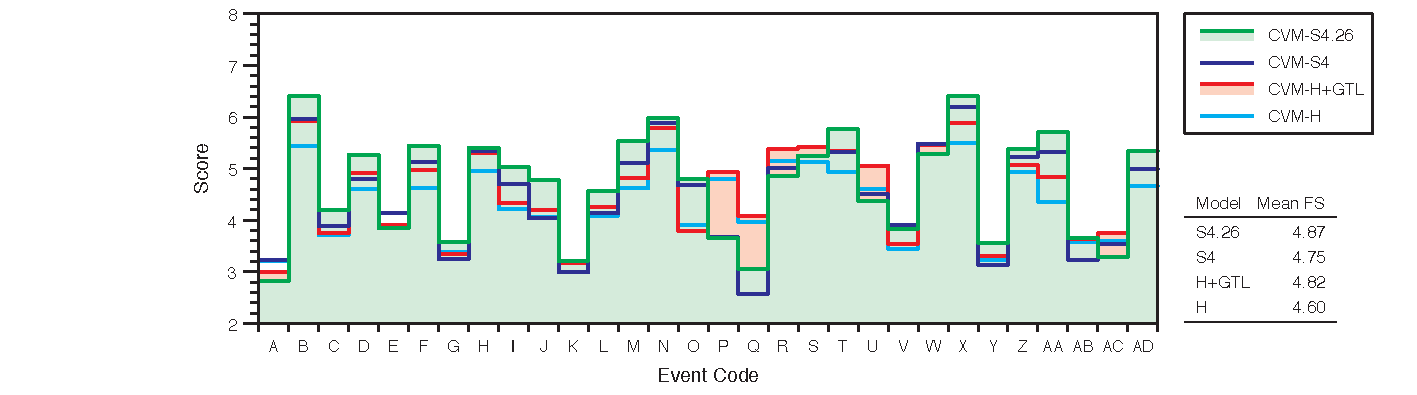
\includegraphics
        [width=\textwidth]
        {figures/pdf/figure-06}
    \caption{Free surface peak horizontal magnitude velocity from simulations for all the events using the velocity model CVM-S4.26. The letter code used to identify each earthquake is shown at the top-left corner along with the event's magnitude, \eqmag{w} (see Table \ref{tab:events}). In each case, the star indicates the epicenter of the event (see also Fig.~\ref{fig:epicenters}). Although smaller and larger values than those shown in the color scale were obtained from the simulations, these were truncated for visual convenience.}
    \label{fig:all.pgvs}
\end{figure*}

\begin{figure*}
    \centering
    \includegraphics
        [width=\textwidth]
        {figures/pdf/figure-07}
    \caption{Free surface peak horizontal magnitude velocity for three representative events (from top to bottom: G, W, and P) using all four velocity models (from left to right: CVM-S4, CVM-S4.26, CVM-H and CVM-H+GTL). The stars indicate the epicenter locations (see Table \ref{tab:events} and Fig.~\ref{fig:epicenters} for reference). In each case, smaller and larger values than those shown in the contour maps were obtained, but truncated for visual convenience.}
    \label{fig:selected.pgvs}
\end{figure*}

Fig.~\ref{fig:selected.pgvs} shows the peak horizontal magnitude of velocity on the free surface for all velocity models, for the particular cases of the 2005 \eqmag{w} 4.42 Fontana, 2007 \eqmag{w} 4.66 Chatsworth, and 2014 \eqmag{w} 5.10 La Habra earthquakes (events G, P, and W, respectively). We select these three events for their location and magnitudes above 4, with well spread response over the simulation domain. The Fontana (G) earthquake epicenter was located in the northern section of the San Jacinto fault zone, not far from the junction with the San Andreas fault zone and the Cucamonga fault (see Fig.~\ref{fig:epicenters}). This earthquake shows clear influence in the area of the San Bernardino basin for all four models, although with some differences. In the case of CVM-S4, for instance, a significant level of the response is channeled into the Chino and the greater Los Angeles basins, as well as far into the Simi and the Santa Clara river valleys. A similar response is seen in the case of CVM-S4.26, but to a lesser extend, with only marginal response in the Santa Monica area. CVM-S4.26 also exhibits lower values southwest and northwest fromt he epicenter than CVM-S4. In the cases of CVM-H and CVM-H+GTL, the ground motion is more localized around the epicentral area. Both models, however, seem to channel more energy along the north flank of the San Andreas Fault and to the south east and south west, in particular along the west edge of the Santa mountains, where both CVM-H and CVM-H+GTL have deeper structures than CVM-S4 or CVM-S4.26 (see Fig.~\ref{fig:hslices} for reference).

In the case of the Chatsworth earthquake, the strongest response concentrates in the Simi and San Fernando valleys, along the Santa Clara river valley and into the Ventura basin. For the simulations done with CVM-S4 and CVM-S4.26, however, a greater amount of energy is channeled west into the Ventura basin and southeast towards the greater Los Angeles area. Both CVM-S4 and CVM-H show some level of basin effects in San Bernardino, an area where CVM-H+GTL shows the least level of amplification of all the models, due to the changes introduced by the GTL model as highlighted in Fig.~\ref{fig:vslices}. Both CVM-H and CVM-H+GTL show a stronger contrast between the Simi and San Fernando valleys and the Los Angeles basin, marked by the influence of the Santa Monica mountains, which seem to be more sharply defined in these two models than in CVM-S4 and CVM-S4.26 (see Fig.~\ref{fig:hslices}).

Last, in the case of the La Habra earthquake, the ground motions are mostly concentrated in the greater Los Angeles basin, though with some significant differences amongst the models. We first note again the fact that the model CVM-H+GTL introduces strong changes in the response of the San Bernardino basin with respect to CVM-H. As in other cases, CVM-H and CVM-H+GTL yield larger ground motions in the area of Irving (see Fig.~\ref{fig:region}) southeast from the epicenter. CVM-S4 and CVM-S4.26, on the other hand, exhibit larger ground motions within the Los Angeles basin itself and in the Chino basin. In turn, CVM-S4.26 yields larger shaking near the San Gabriel valley and mountains, and beyond in the Mojave desert. CVM-S4.26 also exhibits stronger response in the area of the Santa Ana mountains, as a result of the contrast in the model in this area with respect to CVM-S4. Of all four models, CVM-S4 has stronger response in the Ventura basin and CVM-H along the Santa Clara river valley---which likely reflects a better coupling between the crustal structure and faults representation in the model, considering the weak zone along the Santa Clara river due to the presence of the Oak Ridge fault beneath it.

Although not in equal measure for all events, the differences just highlighted were common among the models in the simulation results of other earthquakes. We further analyze the implications of these model discrepancies and their consequence in simulation results through the validation of synthetics against data in the following sections.


